\documentclass[11pt,a4paper]{article}
\usepackage[margin=25mm]{geometry}
\usepackage{fontspec,unicode-math,booktabs,graphicx,hyperref}
\setmainfont{STIXGeneral}\setmathfont{STIX Two Math}\hypersetup{hidelinks}
\setlength{\emergencystretch}{2em}
\title{Group operations: three complete originals}
\author{Human Compression project}\date{Numerical candidate awaiting independent review}
\begin{document}\maketitle
The three Piedade--Tranchida originals N005, N006 and N007 are compared with the whole common theory and every complete application and companion. The written comparison is
\[
\frac{c(N005)+c(N006)+c(N007)}{c(U)+c(A_{005})+c(A_{006})+c(A_{007})}
=\frac{200,891}{158,594}=\mathbf{1.266700}.
\]
The whole declared programme consists of 23 mathematical or validation files and both complete required decoding drivers. Including it gives
\[
\frac{200,891}{158,594+403,848}
=\frac{200,891}{562,442}=\mathbf{0.357176}.
\]
These are separate comparisons. The source historical software and complete retained external proofs remain unpriced. Thus neither fraction is a fully priced comparison of all external mathematical work.

\begin{center}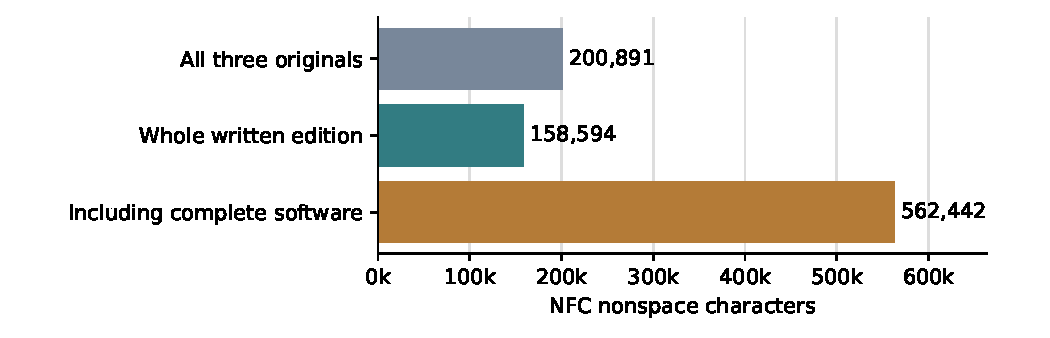
\includegraphics[width=\linewidth]{costs.pdf}\end{center}

\begin{center}\begin{tabular}{lrrr}\toprule
Complete matched papers & Original & Application & Conditional factor\\\midrule
N005: group operations & 122,002 & 49,595 & 2.459966\\
N006: wreath and semidirect products & 56,001 & 38,479 & 1.455365\\
N007: diagonal twistings & 22,888 & 12,305 & 1.860057\\\bottomrule
\end{tabular}\end{center}
These conditional figures are $c(N_i)/c(A_i)$ \emph{after acquiring the whole common theory, all 23 files and both decoding drivers}, together with the required external data. Every local proof, companion and reference remains charged. There is no overlap discount between separate topics.

Primary unit: selected calibrated NFC nonspace characters. The encoded graphic-event substitutions are proxies for components, not complete geometry or literal Unicode extraction.
\newpage
\section*{The complete paper sequence}
The common paper has 21 pages and costs 58,215 characters. N005 has 18 pages; N006 comprises all three papers of 8, 5 and 4 pages; N007 has 5 pages. These six scientific documents total 61 pages. The three originals total 94 pages. References and front matter remain included on both sides.

\begin{center}\begin{tabular}{lrrrr}\toprule
Stage & New written cost & Written total & New original & Original total\\\midrule
U & 58,215 & 58,215 & 0 & 0\\
N005 & 49,595 & 107,810 & 122,002 & 122,002\\
N006 & 38,479 & 146,289 & 56,001 & 178,003\\
N007 & 12,305 & 158,594 & 22,888 & 200,891\\\bottomrule
\end{tabular}\end{center}
\begin{center}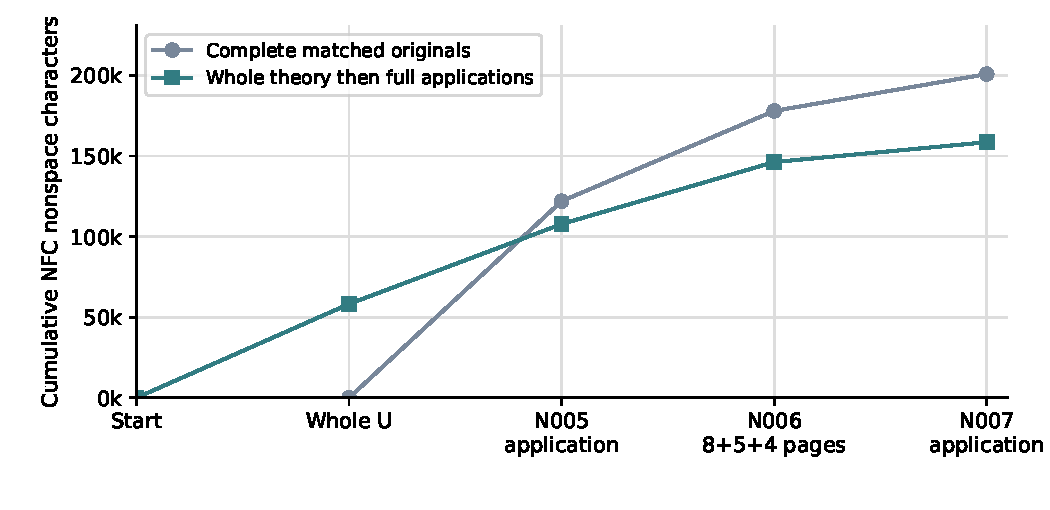
\includegraphics[width=\linewidth]{acquisition.pdf}\end{center}
The ordering displays whole documents, not theorem-node costs or an empirical learning curve. The initial source entry is zero because no matched original has yet been accumulated; it does not assign zero cost to historical common theory. The whole software bundle is shown separately on page~1 and is prepaid for the conditional comparisons.

\begin{center}\begin{tabular}{lrr}\toprule
Whole files & Nonspace characters & Raw bytes\\\midrule
23 mathematical/validation files & 392,833 & 448,737\\
2 required decoding drivers & 11,015 & 12,271\\
5 operational drivers (separate) & 27,575 & 30,275\\
3 Lean files (separate) & 5,820 & 7,829\\\bottomrule
\end{tabular}\end{center}
Seventeen mathematical files supply finite premises or saved witnesses; six are validation. Large saved permutations receive no discount. The 17 Lean declarations are scoped partial evidence, with no new N005 formalization.
\newpage
\section*{Sensitivity and retained costs}
\begin{center}\begin{tabular}{lrrrr}\toprule
NFC nonspace convention & Originals & Written & Written factor & With software\\\midrule
Literal full extraction & 203,841 & 158,676 & 1.284637 & 0.362369\\
Literal selected extraction & 200,862 & 158,594 & 1.266517 & 0.357125\\
Calibrated selected & 200,891 & 158,594 & 1.266700 & 0.357176\\
Graphic proxies removed & 200,313 & 158,594 & 1.263055 & 0.356149\\\bottomrule
\end{tabular}\end{center}
The raw rows preserve extraction without glyph substitutions. The text-only sensitivity removes only identified graphical proxies. The input audit reconciles actual PDF font dictionaries, encodings and occurrences, including 20 visible N005 strokes extracted as carriage returns. Full drawing structure, placement and curvature remain unmeasured.

\begin{center}\begin{tabular}{lrrrr}\toprule
Calibrated selected unit & \multicolumn{2}{c}{Written factor} & \multicolumn{2}{c}{With software}\\
& NFC & NFKC & NFC & NFKC\\\midrule
Whitespace tokens & 1.366751 & 1.369412 & 0.709983 & 0.711365\\
Alphanumeric units & 1.409743 & 1.409743 & 0.418808 & 0.418808\\
Nonspace characters & 1.266700 & 1.266325 & 0.357176 & 0.357147\\
Collapsed-space characters & 1.284635 & 1.284799 & 0.394531 & 0.394647\\
Collapsed-space UTF-8 bytes & 1.219405 & 1.335426 & 0.404567 & 0.415950\\\bottomrule
\end{tabular}\end{center}
The JSON/CSV contain all 30 ordinary settings and 10 text-only settings, with 200 exact fractions. Printed hyphens remain counted. Only exact running furniture is removed. The audit covers 11 PDFs and 161 pages, including two partial printed alternatives; this is not a 161-page replacement.

There is \emph{no complete printed programme factor}. The 4-page N005 appendix (8,564 characters) replaces only three named raw files; the 2-page N007 appendix (3,161) replaces only its one validation file. The remaining whole files and decoders cannot be omitted. Both printed alternatives are inventoried, never added to the same raw files.

Four required Atlas representation files occupy 21,960,689 bytes; sixteen listed installed catalogue/algorithm files occupy 2,516,249 bytes. These storage figures are separate from text costs. Binary/decoded and compressed/decompressed forms are alternatives. Named-group identification, maximal-subgroup classification, Coxeter and Artin theory, normal forms, Bass--Serre theory and affine-reflection inputs remain retained. Full external proofs, graphics, historical software and complete formalization have unknown cost, not zero cost.

All $81+27+32$ source dispositions and their corrections/exclusions are preserved. The unrestricted nonfirm HNN claim is not recovered, and unresolved general questions are not answered by these numbers. The later separate Fischer exception certificates are outside this comparison. This packet changes no source, question or formal credit and does not rerun source extraction, GAP or Lean.
\end{document}
